%%%%%%%%%%%%%%%%%%%%%%%%%%%%%%%%
%------------------------------%
%%%%%%%%%%%%%%%%%%%%%%%%%%%%%%%%
\section{Supplementary material}
%%%%%%%%%%%%%%%%%%%%%%%%%%%%%%%%
%------------------------------%
%%%%%%%%%%%%%%%%%%%%%%%%%%%%%%%%

\begin{figure}[H]
    \centering
    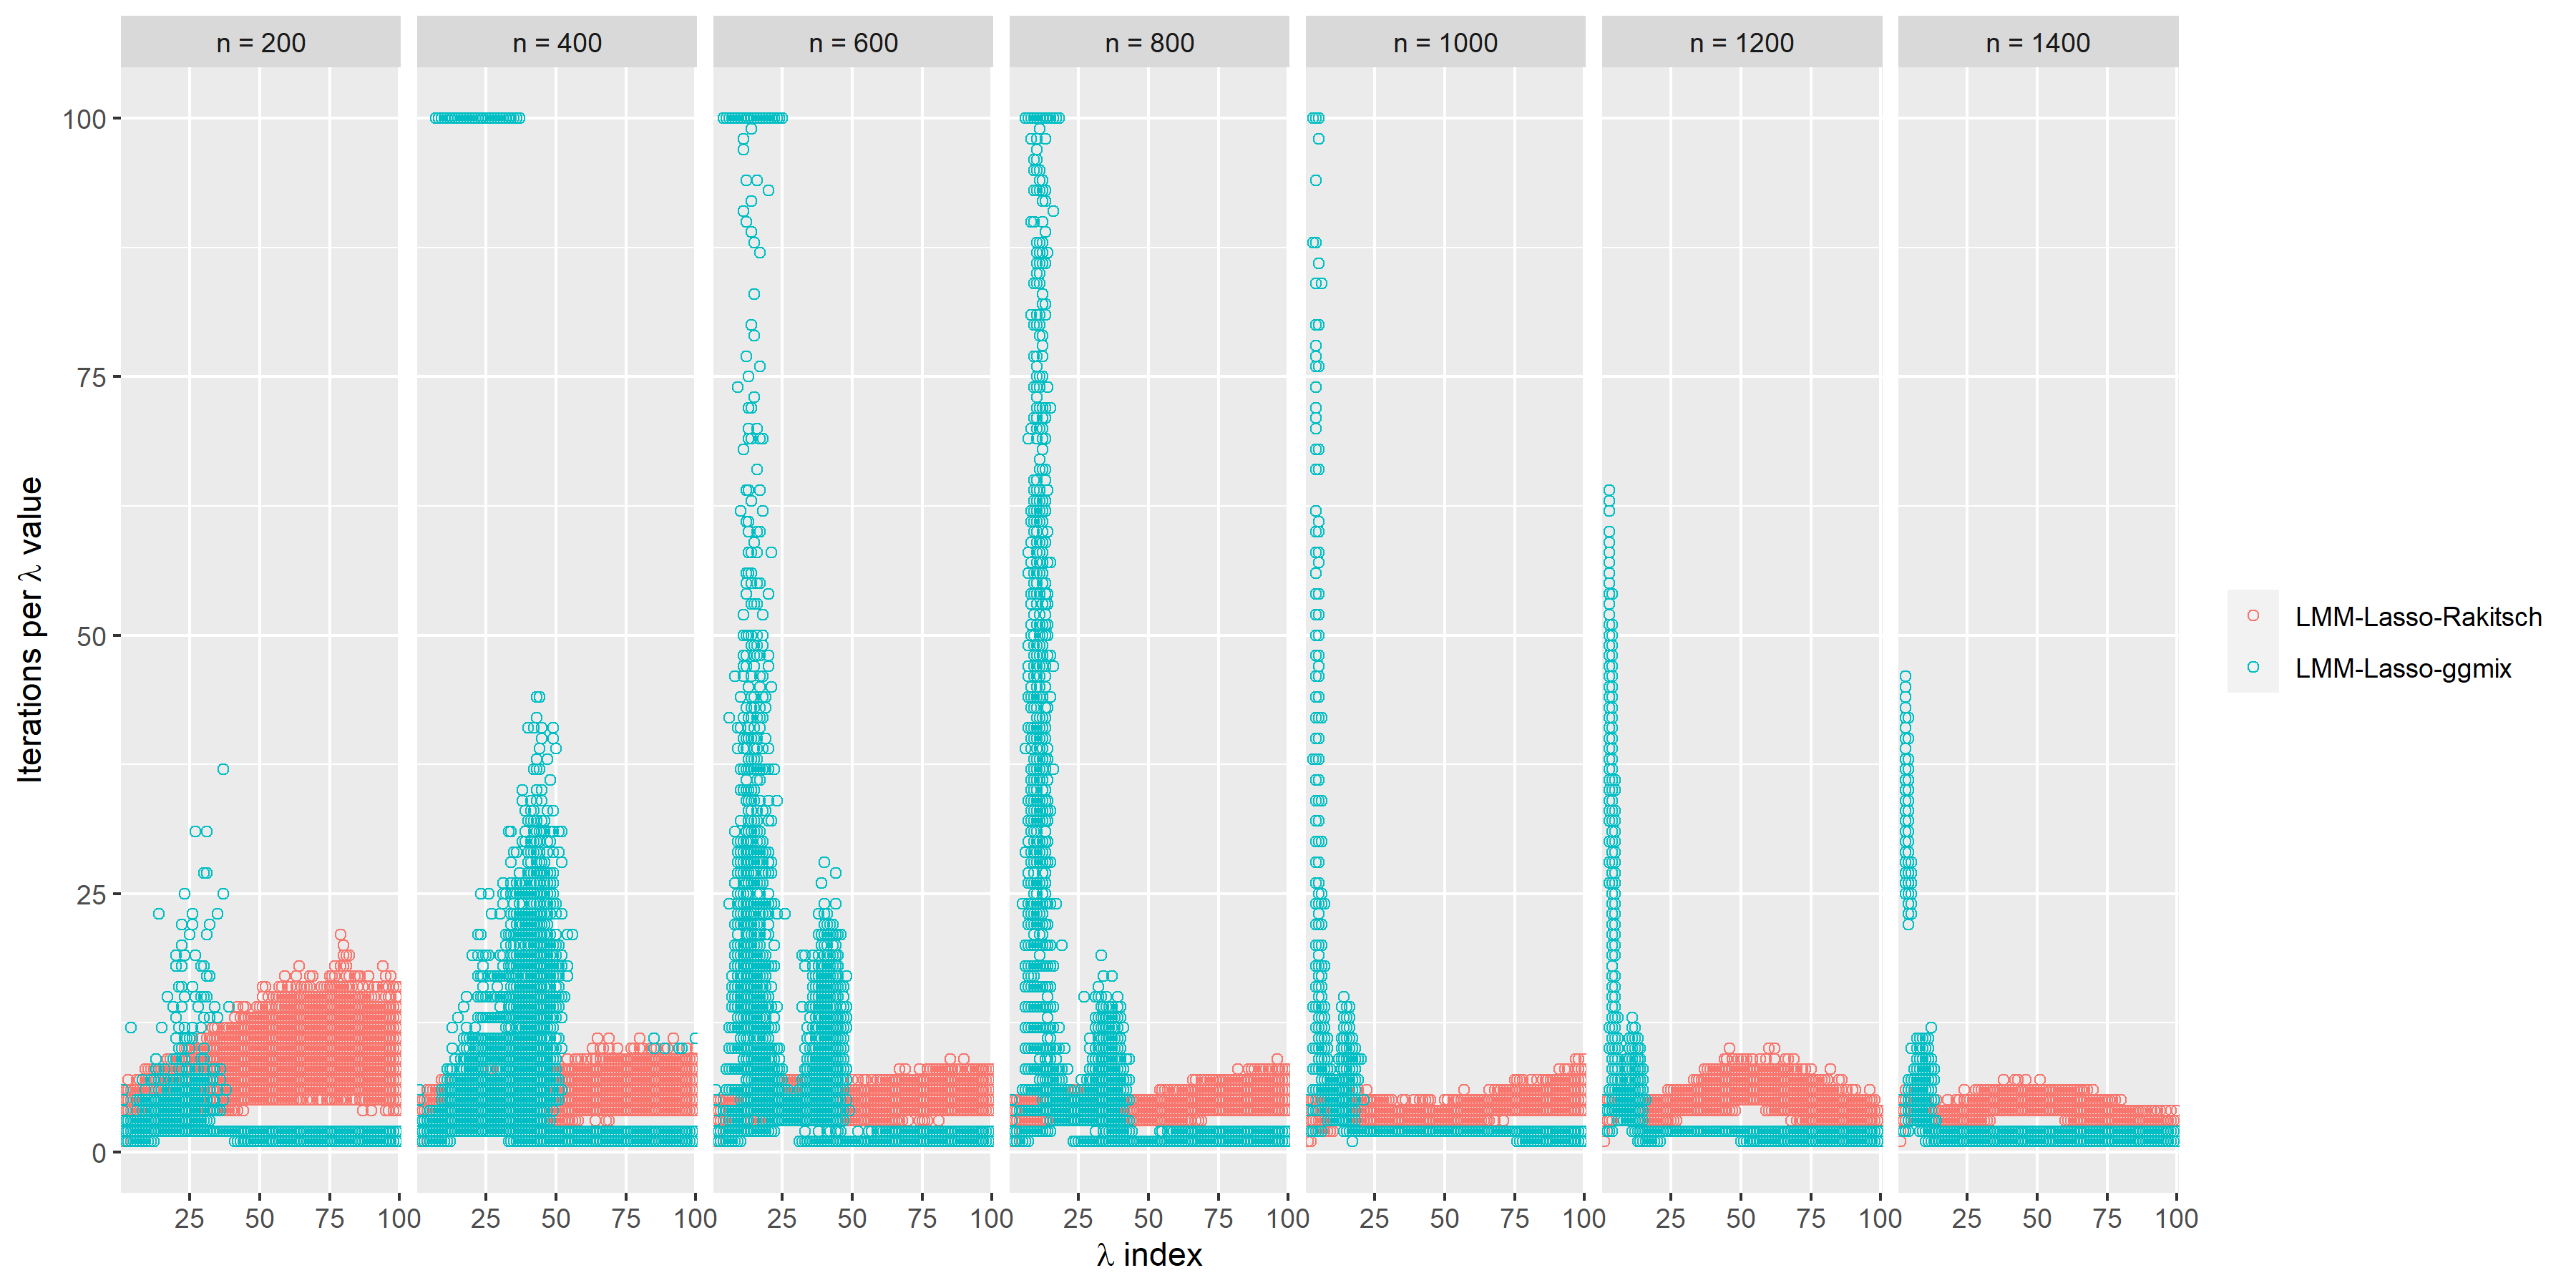
\includegraphics[scale = 0.45]{figures/niter_perLambda_point.png}
    \caption{The number of iterations per $\lambda$ value for LMM-Lasso-Rakitsch and LMM-Lasso-ggmix across varying sample sizes with Independent Subpopulations data, coarse subpopulation structure, $\eta = 0.8$, and $\xi = 0.8$, and dichotomous-discordant environmental effect structure. Note that 100 is the maximum number of iterations for both implementations of LMM-Lasso, so that numerous incidences of 100 iterations may indicate lack of model convergence.}
    \label{fig:s4}
\end{figure}